\chapter{設計}
\label{chap:sekkei}

本章ではハイパー楽譜システムの要件と設計について述べる。

\newpage

\section{要件}
前章で整理した楽譜の問題点を踏まえた上で、ハイパー楽譜システムの要件を整理する。
\begin{enumerate}
    \item 楽譜を簡単に編集できる\\
    メモを取るような気軽さで楽譜を書くことができ、新規作成/既存楽譜の編集両方を簡単に行える。
    \item メモなどの情報を自在に書ける\\
    テキストで楽譜を記述でき、ハイパーテキストのようなフォーマットの中で楽譜以外の情報も一緒に管理できる。
    \item ハイパーリンクを利用できる\\
    楽譜上の要素やテキストに対してハイパーリンクを設定でき、関連情報に素早くアクセスできる。
\end{enumerate}
この要件を満たす楽譜システムは、ハイパーテキストの編集環境であるWikiと、テキストベースの楽譜記述言語の組み合わせによって実現できる。

\section{ハイパー楽譜システム}
本研究で提案するハイパー楽譜システムの基本構成と使い方を解説する。

\subsection{基本構成}
ハイパー楽譜システム(図\ref{hs})はWikiであるScrapbox\footnote{\textsf{https://scrapbox.io}}と、楽譜記述言語のABC記譜法\footnote{\textsf{http://abcnotation.com}}(以下ABC)によって構成されている。

\begin{figure}[H]
    \centering
    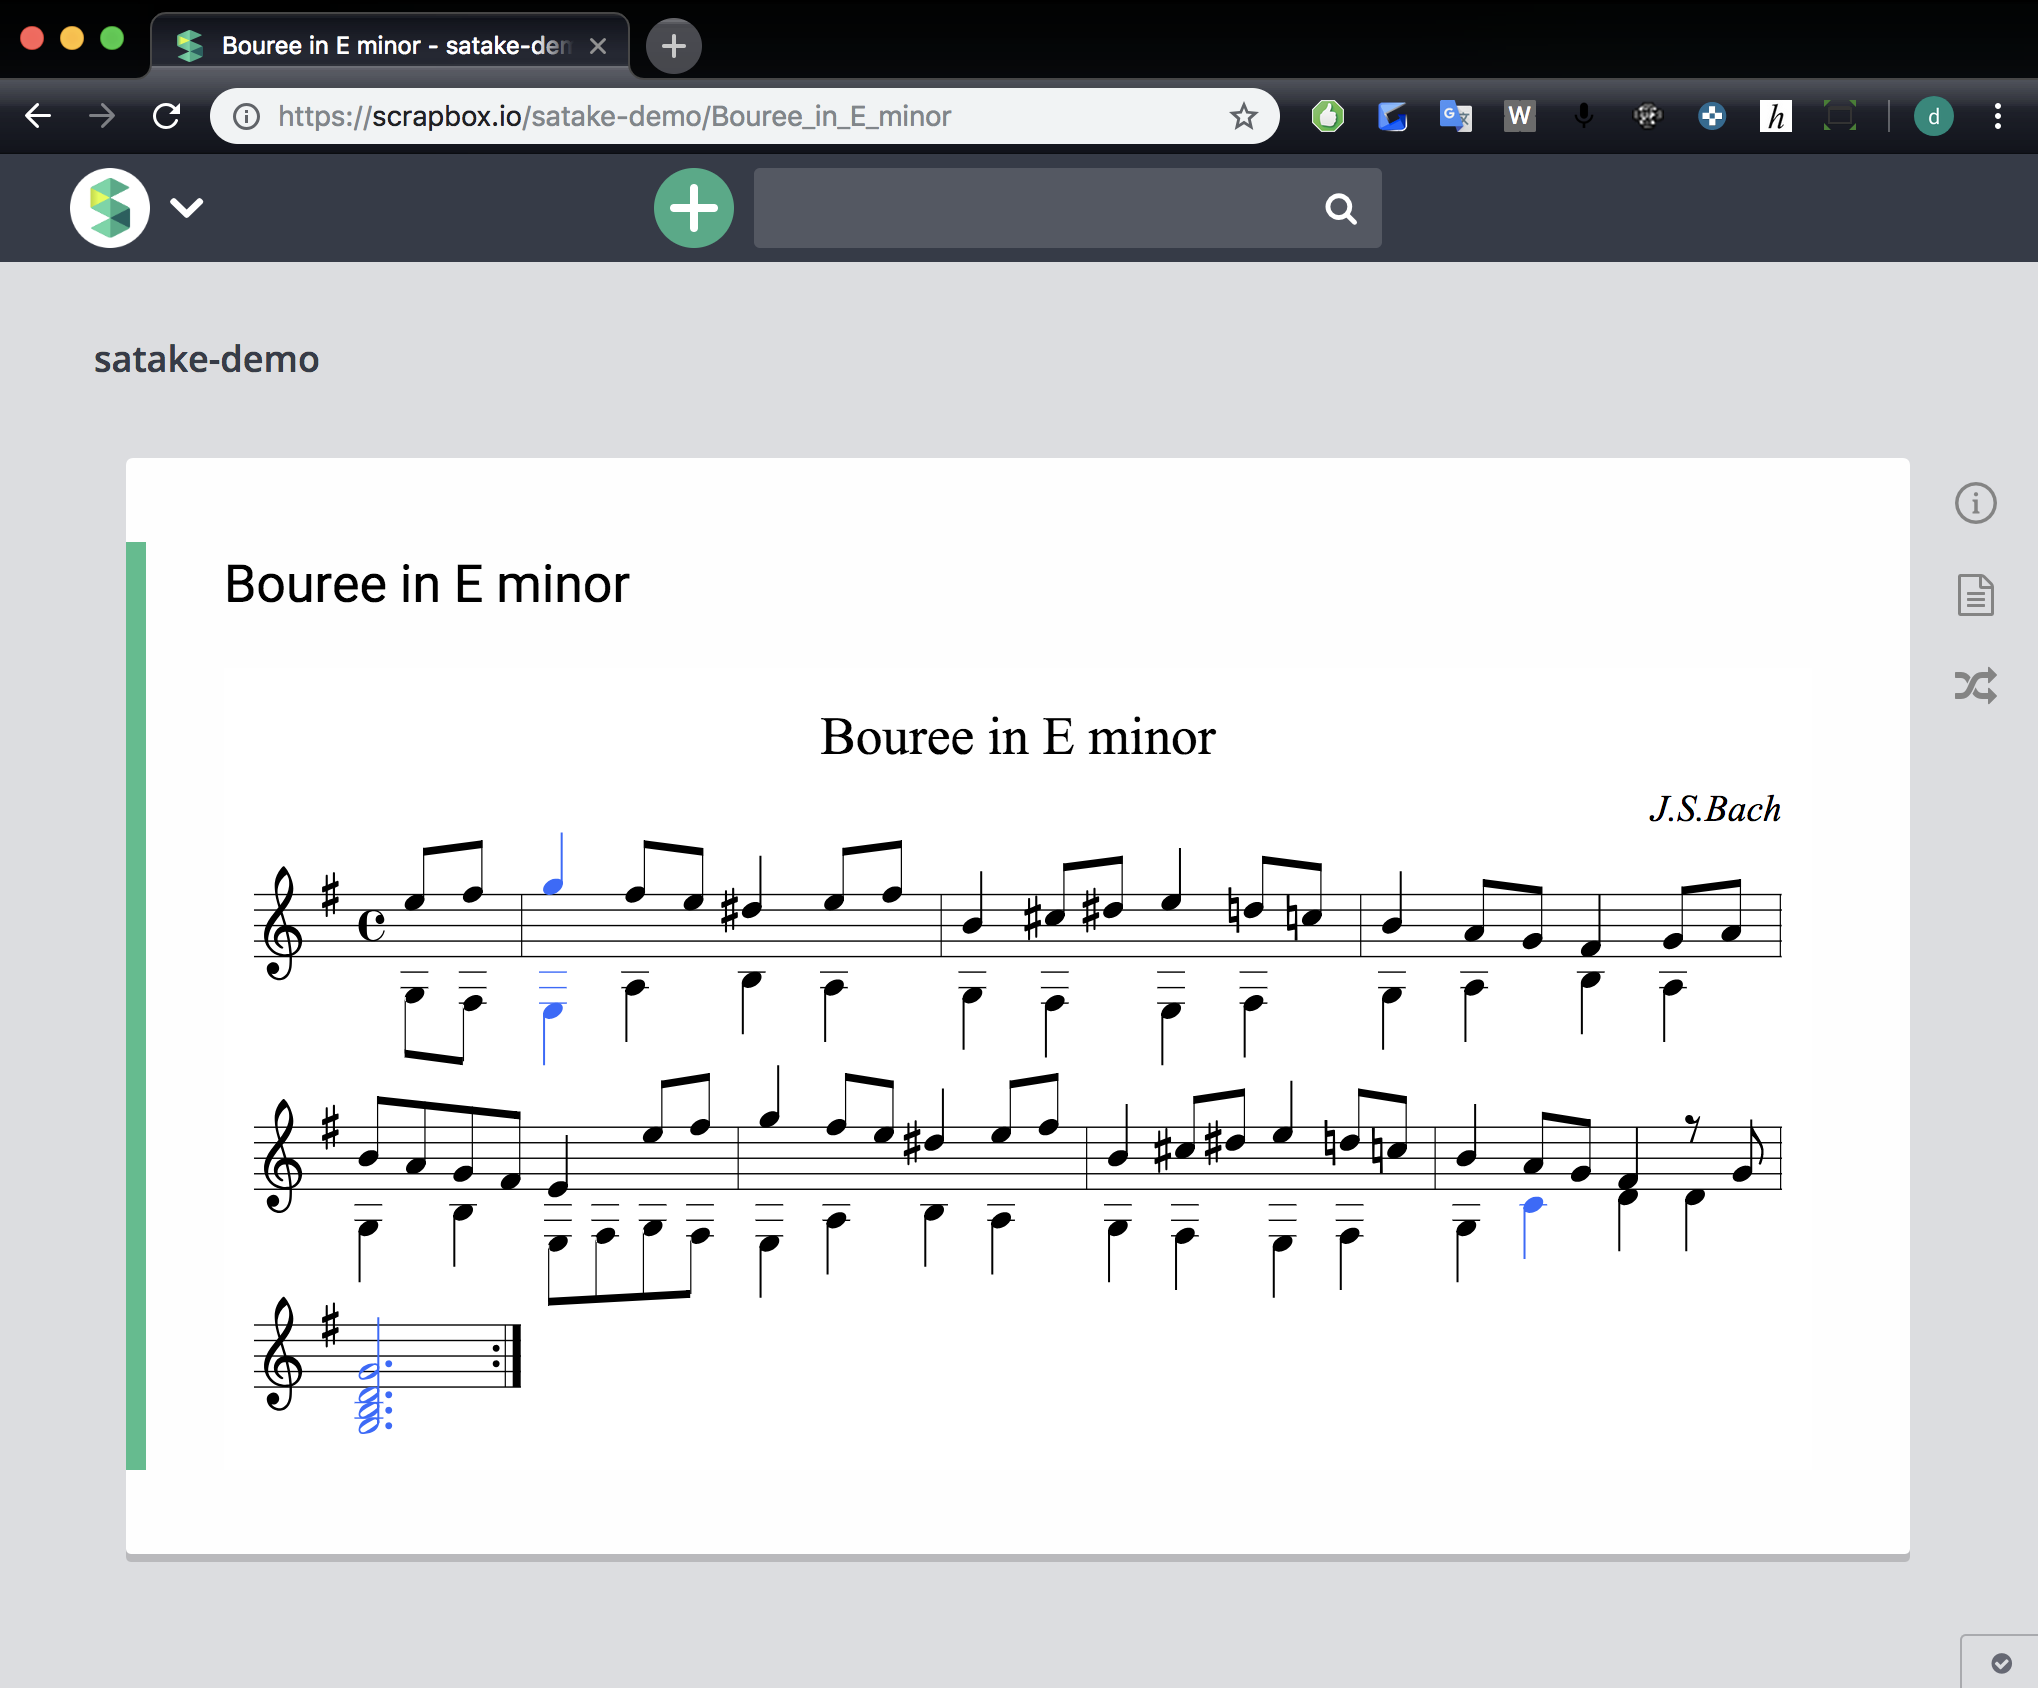
\includegraphics[width=10cm]{images/hyperscore.png}
    \caption{ハイパー楽譜システム上で書かれた楽譜}
    \label{hs}
\end{figure}


\paragraph*{Scrapbox}
Scrapbox(図\ref{scrap})はGyazz\cite{Gyazz}をベースにして開発された、Nota\footnote{\textsf{https://www.notainc.com/ja}}社が運営しているWikiである。
他のシステムには存在しない、ハイパー楽譜システムとして利用するのに最適な特徴を持つ。

\begin{itemize}
    \item シンプルで柔軟な記法をもつWYSIWYGエディタ

    入力/改行/段落/箇条書きといった基本的なテキスト編集を見たまま行える。
    またリンクやマルチメディアの埋め込みには\texttt{[]}記法のみで対応でき、他に様々な記法を覚える必要がない。

    \begin{itembox}[l]{\texttt{[]}記法}
        \begin{tabbing}
            ********************************* \= ********************** \kill
            \texttt{[ページ名]} \> 同一Wiki内ページへのリンク\\
            \texttt{[URL]} \> 外部リンク\\
            \texttt{[画像URL]} \> 画像埋め込み\\
            \texttt{[音声URL]} \> 音声埋め込み\\
            \texttt{[YouTube/VimeoURL]} \> 動画埋め込み\\
            \texttt{[GoogleMapsURL]} \> 地図埋め込み
        \end{tabbing}
    \end{itembox}

    \item 関連ページリスト

    Scrapboxページの下部には
    \begin{itemize}
        \item 別ページへのリンク
        \item 別ページからのリンク
        \item リンク先ページがリンクしているページ
    \end{itemize}といった関連ページリスト(図\ref{related})が表示され、どのような情報と関連するのか一目瞭然に分かる。

    \item リアルタイム共同編集

    Scrapboxでは複数人による共同編集だけでなく、Googleドキュメント\footnote{\textsf{https://www.google.com/intl/ja\_jp/docs/about}}のようなリアルタイム編集作業をコンフリクトすることなく行うことが可能である。
\end{itemize}

\begin{figure}[H]
    \centering
    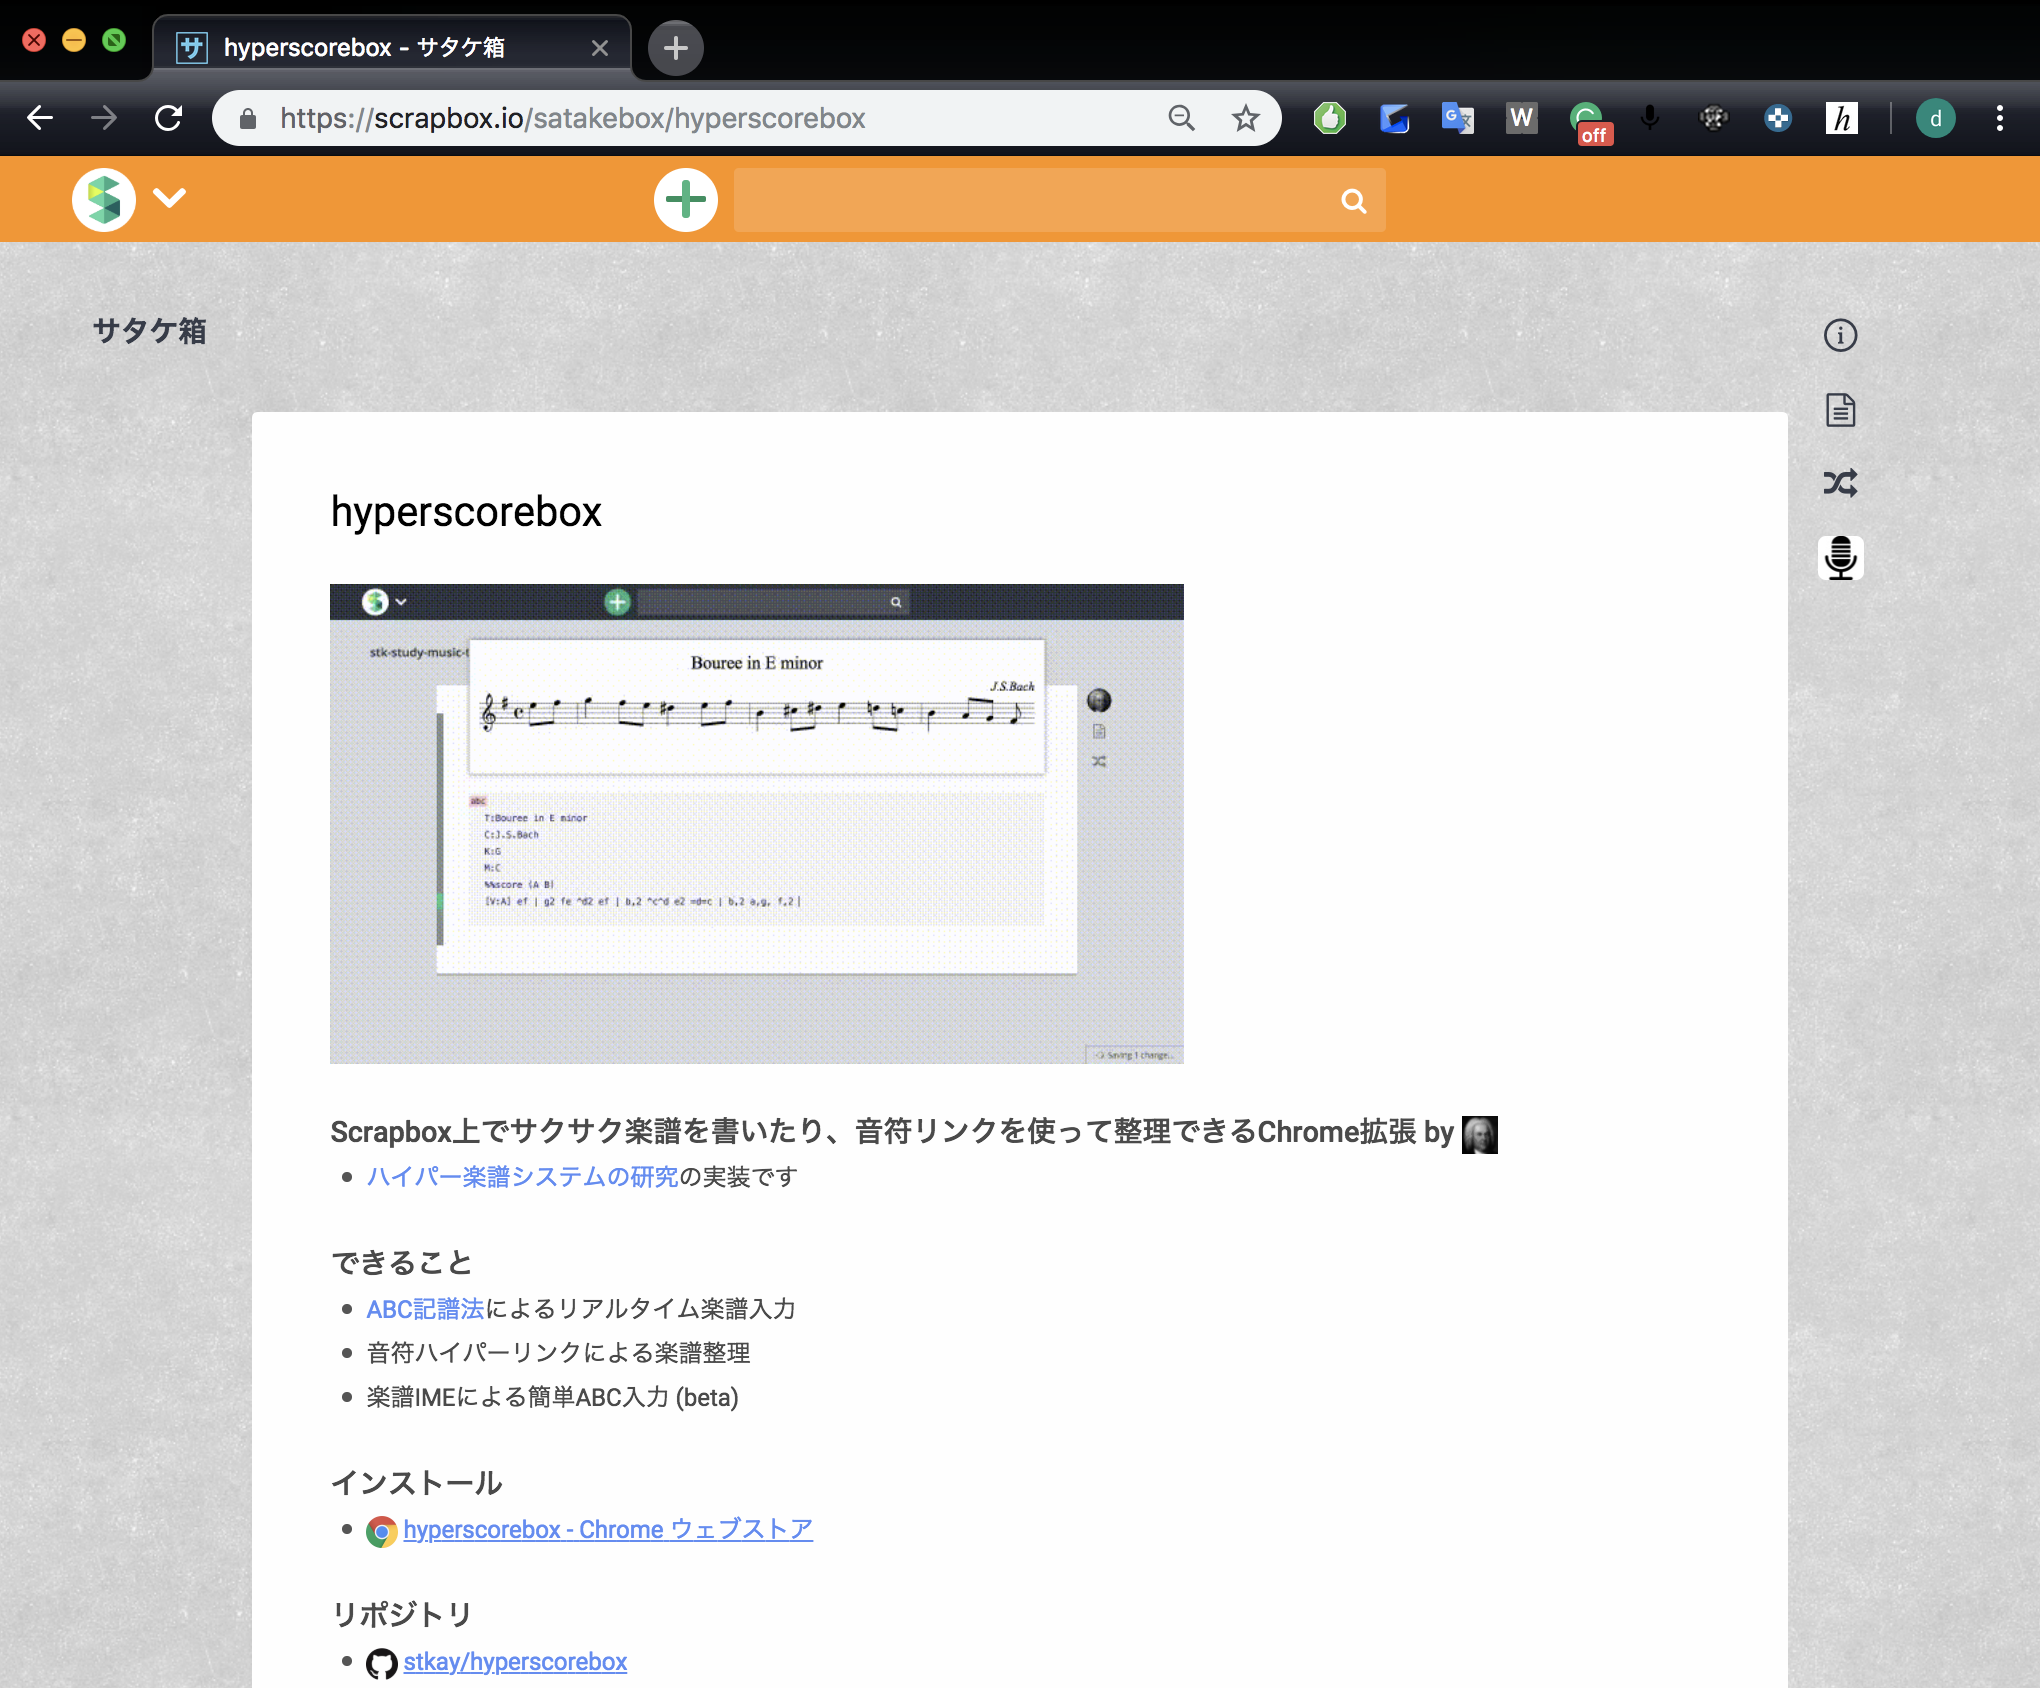
\includegraphics[width=10cm]{images/scrapbox.png}
    \caption{Scrapboxの画面}
    \label{scrap}
\end{figure}

\begin{figure}[H]
    \centering
    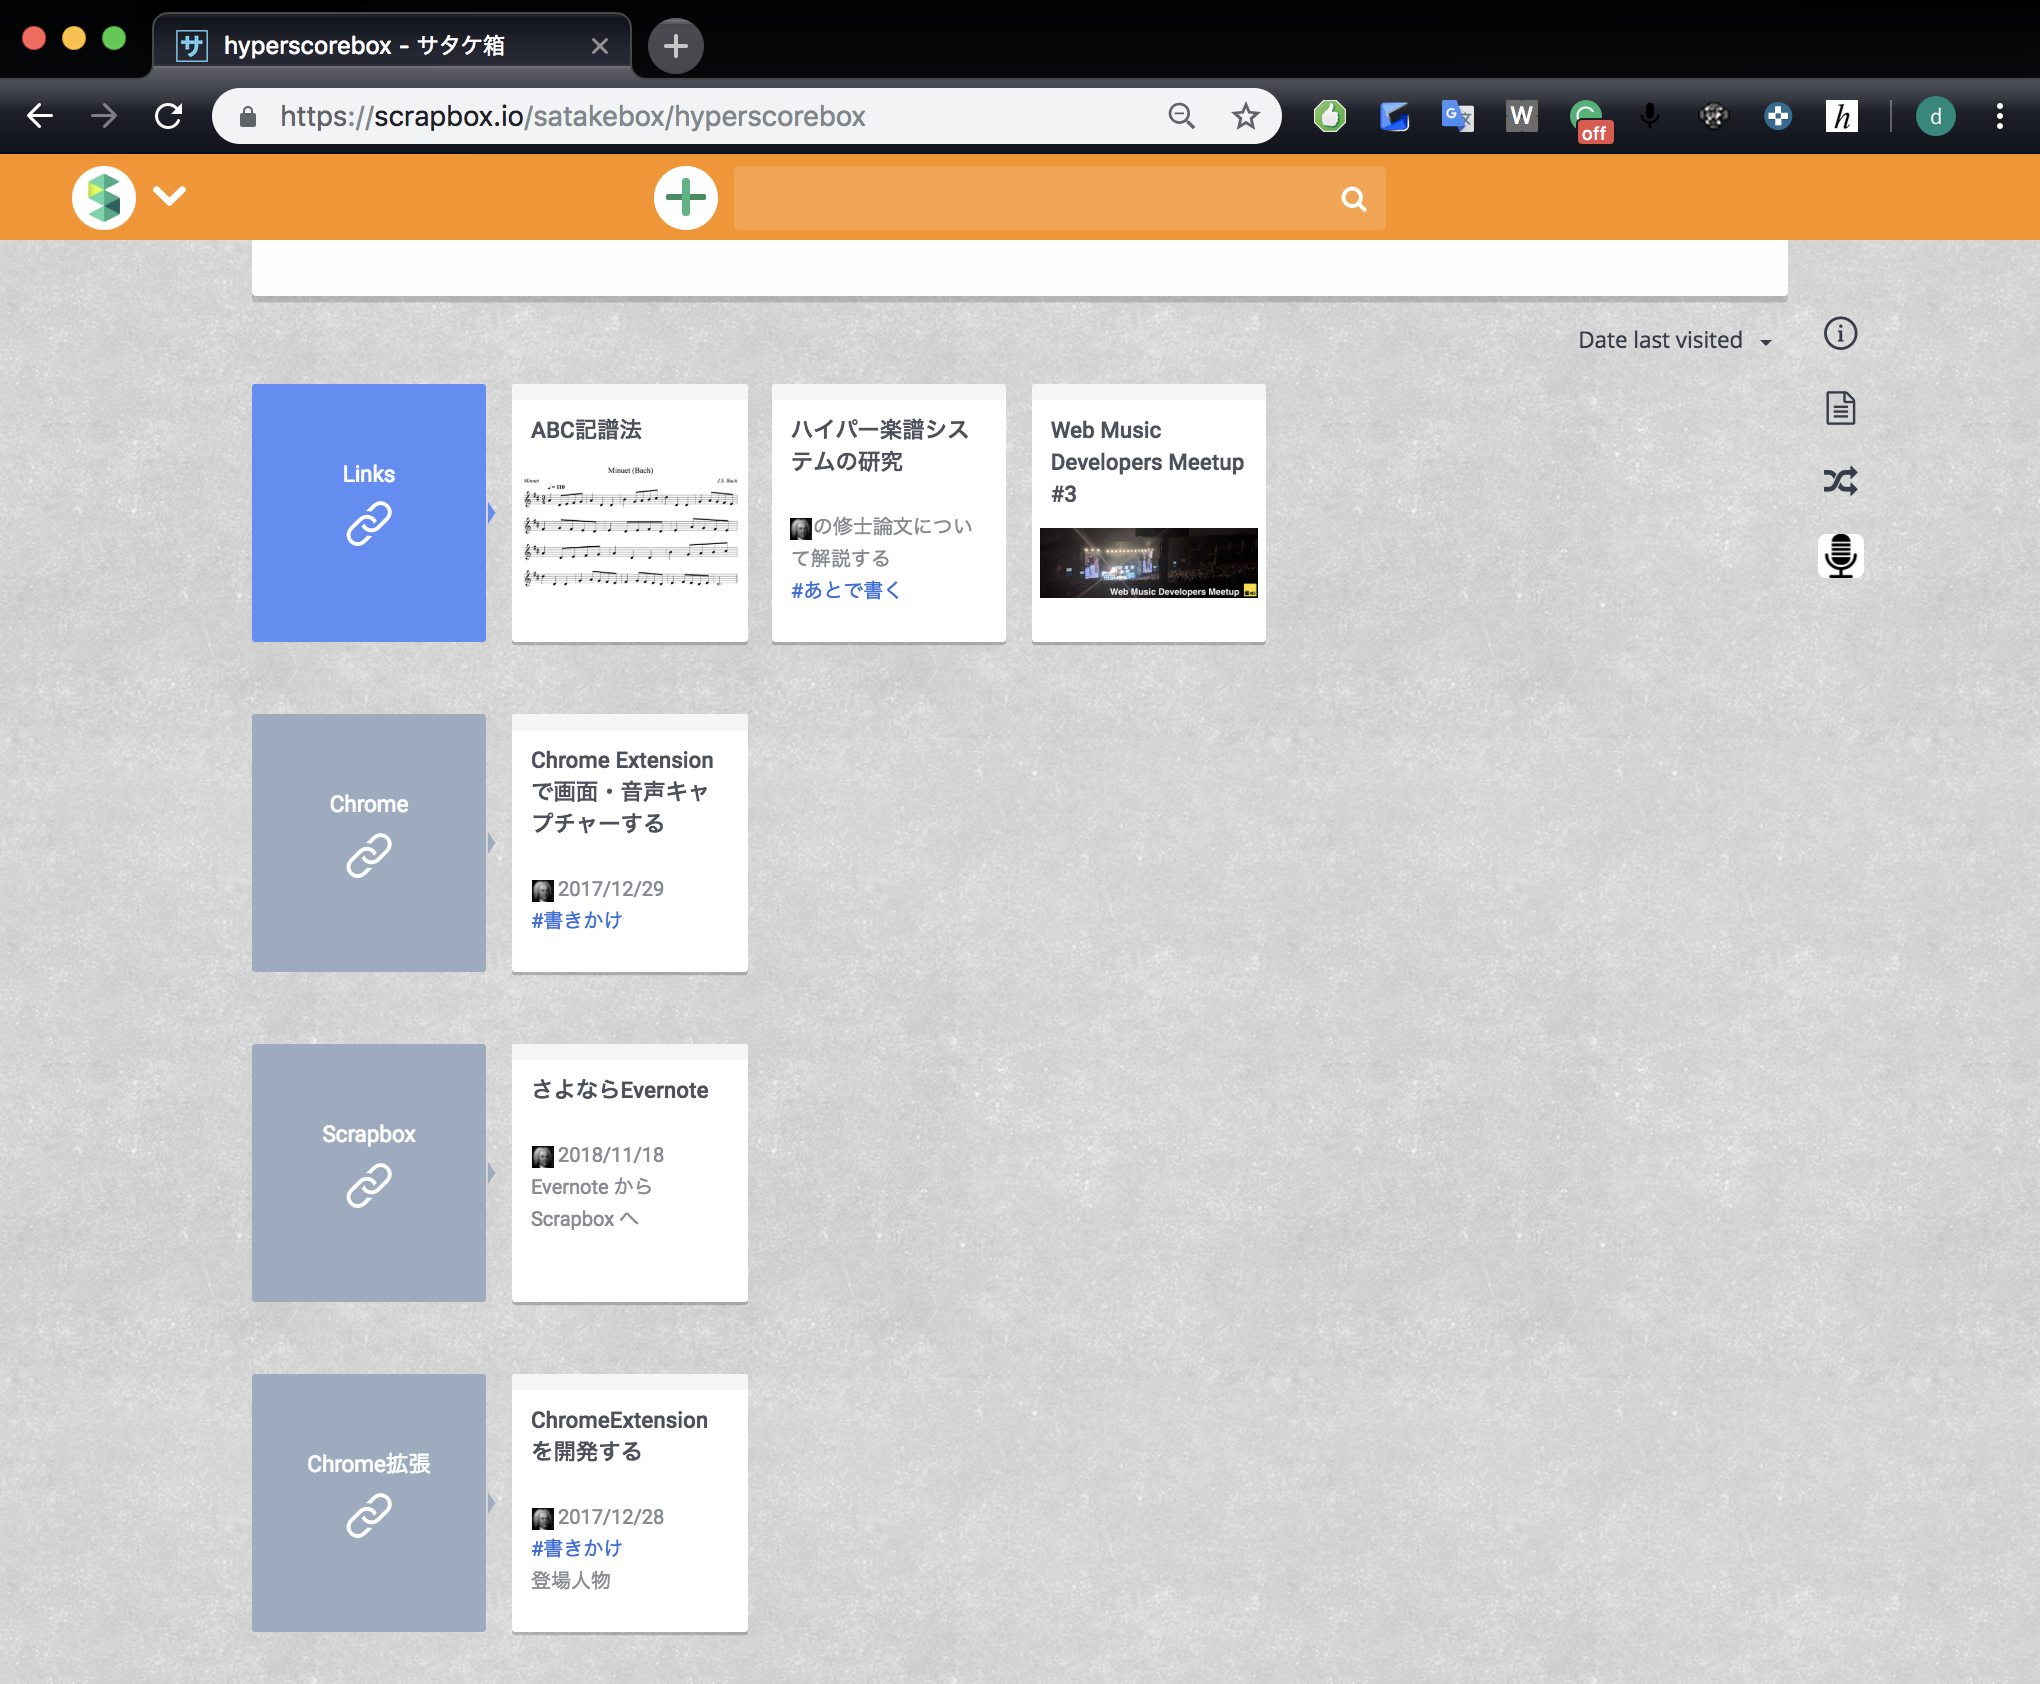
\includegraphics[width=10cm]{images/related.png}
    \caption{関連ページリスト}
    \label{related}
\end{figure}

\paragraph*{ABC}
ABCはプレーンテキスト形式の楽譜記述言語で、\texttt{c}が「ド」を表すシンプルな記法(ソースコード\ref{abctext})を持つ。
大規模で複雑な楽譜(図\ref{complex})の記述も可能で、幅広いシーンで利用可能である。
利用者コミュニティ\footnote{\textsf{https://groups.yahoo.com/neo/groups/abcusers/info}}が活発でバージョンのアップデートが頻繁に行われていたり、ユーザーによる譜例が多く公開されていることから信頼できるフォーマットである。
ブラウザからはJavaScriptライブラリのabcjs\footnote{\textsf{https://abcjs.net/}}が利用でき、既存の楽譜システムと比較しても遜色のない綺麗な楽譜を出力することが可能である。

\begin{lstlisting}[caption=「ド」を表すABC, label=abctext]
    c
\end{lstlisting}
\begin{figure}[H]
\centering
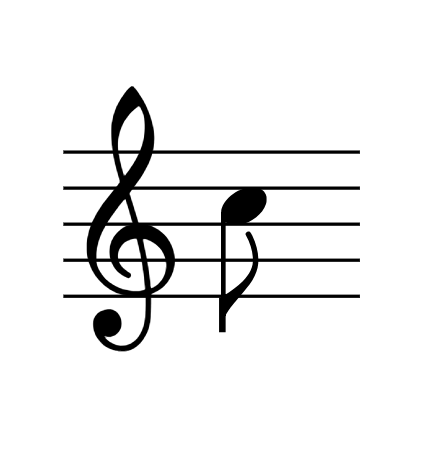
\includegraphics[width=2cm]{images/c.png}
\caption{「ド」の譜例}
\label{abcnote}
\end{figure}

\begin{figure}[H]
\centering
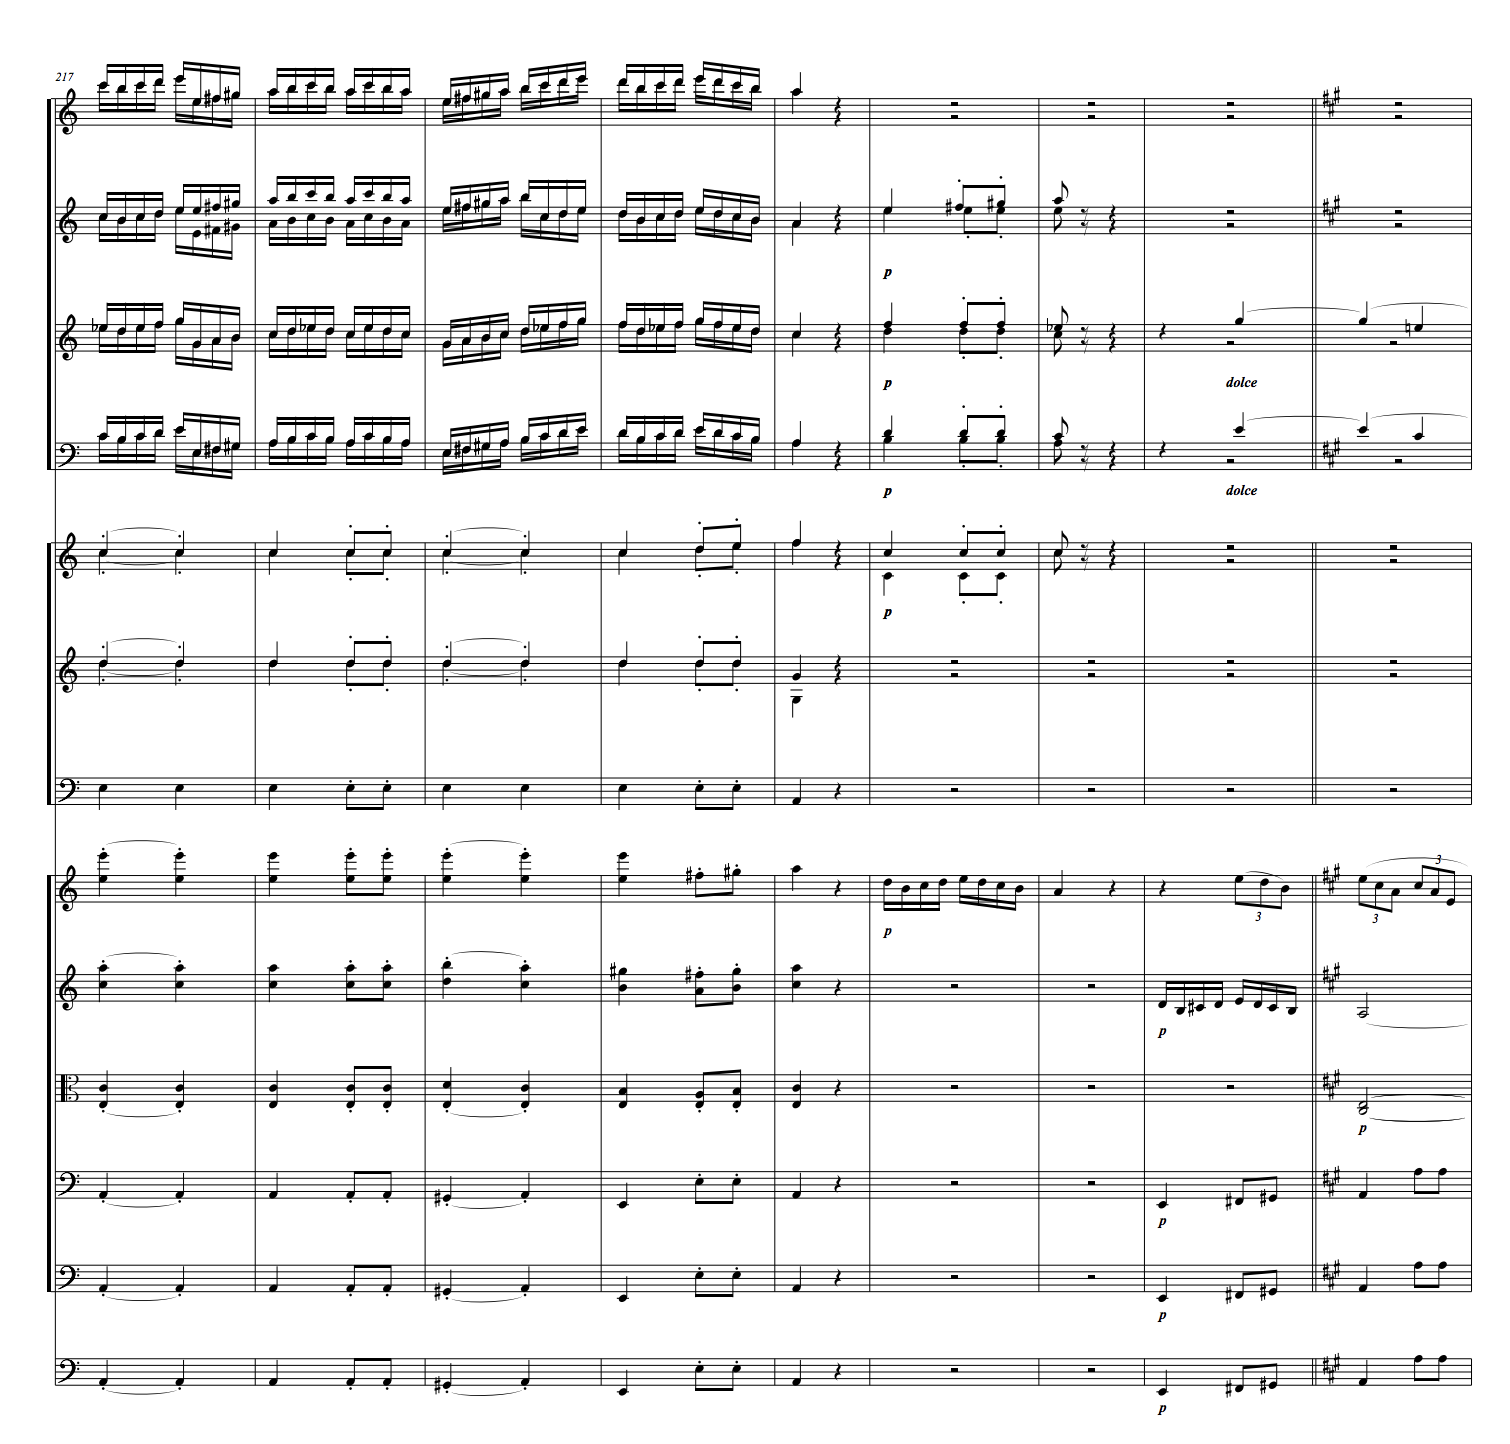
\includegraphics[width=10cm]{images/complexabc.png}
\caption{複雑な楽譜の例}
\label{complex}
\end{figure}


\subsection{使い方}
\paragraph*{楽譜を書く}
Scrapbox上で\texttt{code:*.abc}という行に続けてABCテキストを書くとABC記述の真上に楽譜画像が表示され(図\ref{editingabc})、楽譜を確認しながらリアルタイムに編集できる。
楽譜やABCの領域外をクリックするとABC記述が隠れ、楽譜のみが表示される(図\ref{editedabc})。

\begin{figure}[H]
\centering
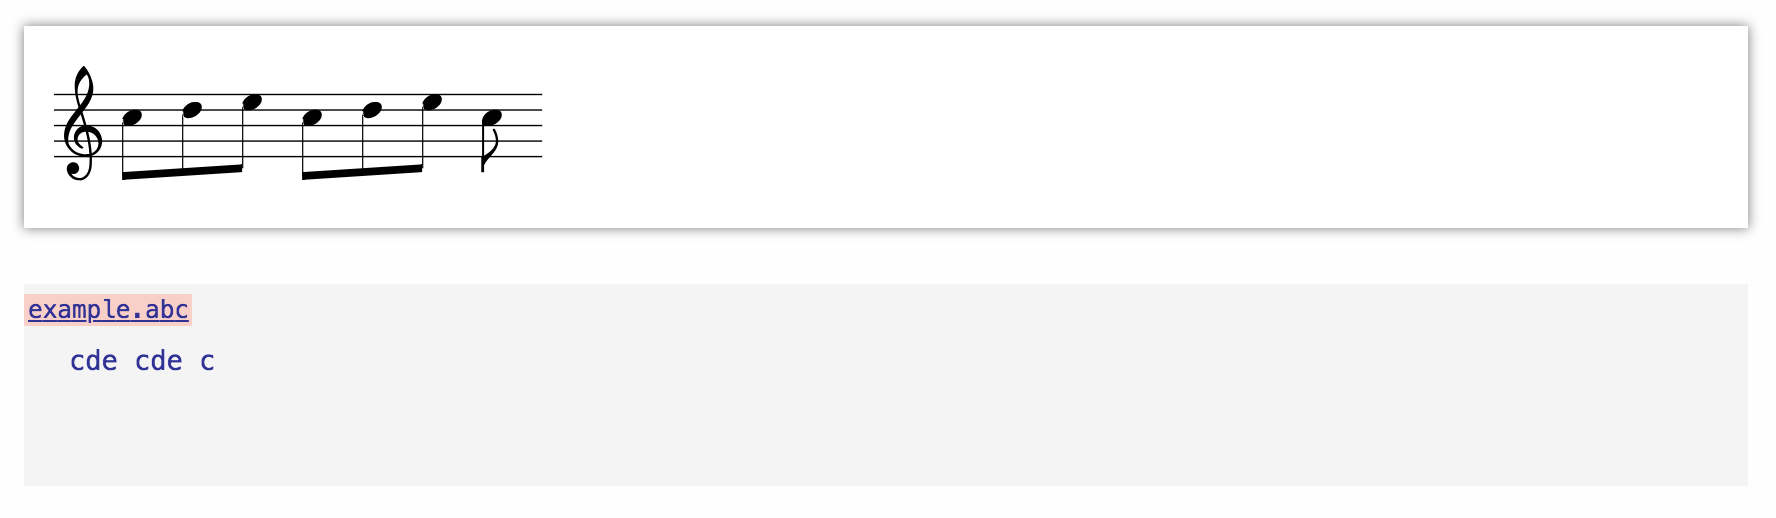
\includegraphics[width=10cm]{images/editingabc.png}
\caption{編集中の楽譜}
\label{editingabc}
\end{figure}

\begin{figure}[H]
\centering
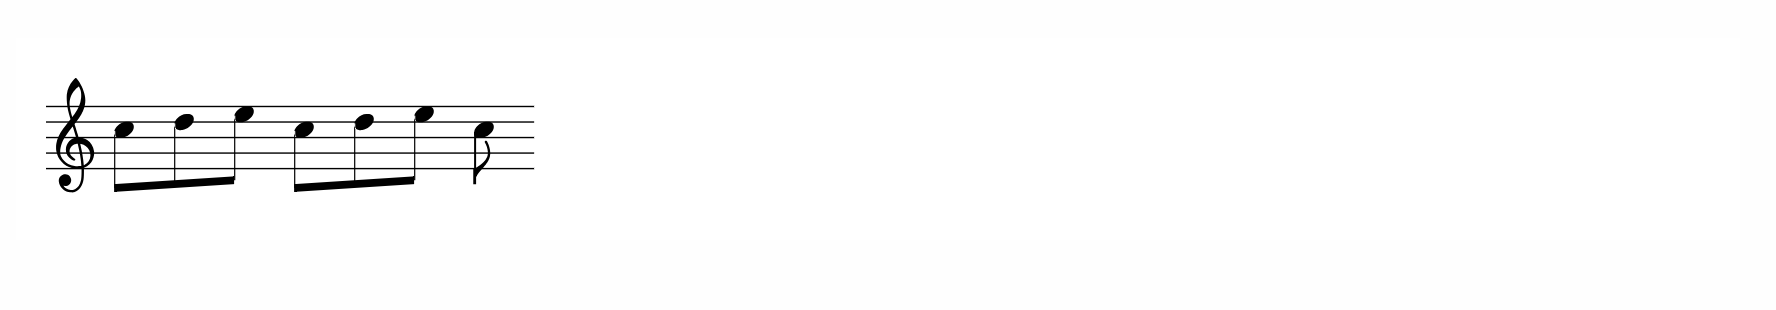
\includegraphics[width=10cm]{images/editedabc.png}
\caption{編集後の楽譜}
\label{editedabc}
\end{figure}


\paragraph*{音符など以外の情報を書く}
楽譜領域以外では標準のScrapbox記法を利用できるので、自在にテキストを書いたり、マルチメディアを埋め込むことができる(図\ref{scoreandtext})。

\begin{figure}[H]
\centering
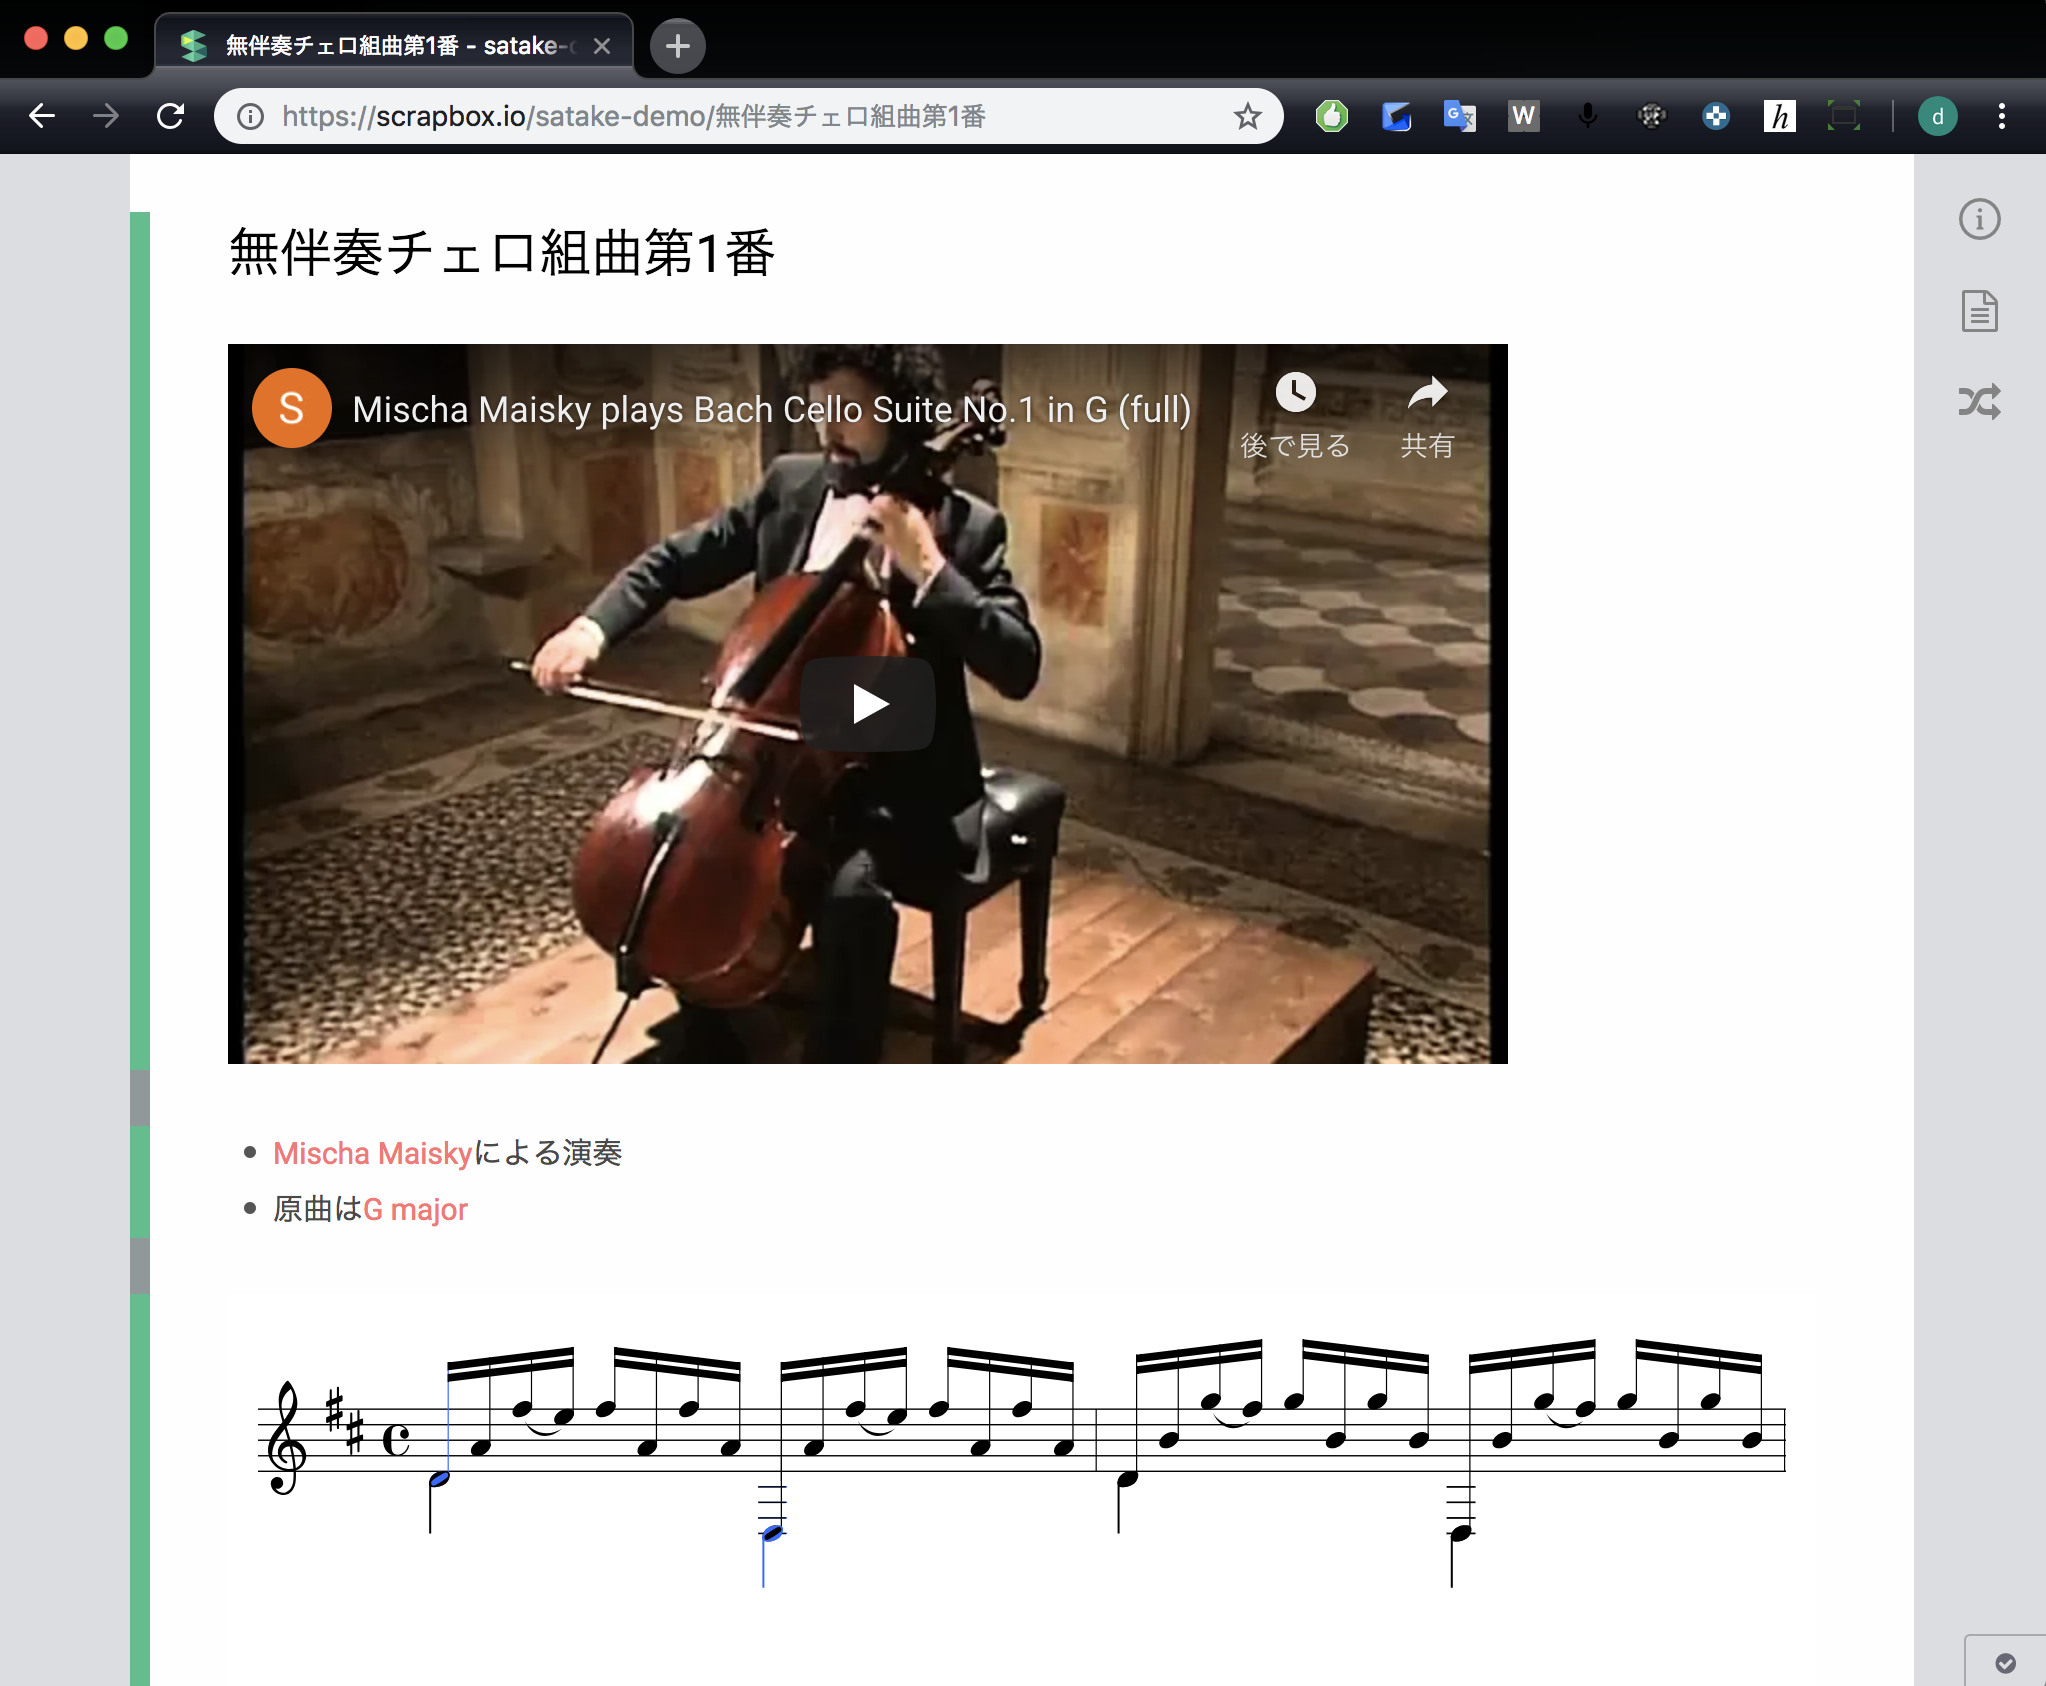
\includegraphics[width=10cm]{images/scoreandtext.png}
\caption{楽譜にテキストや動画が埋め込まれた例}
\label{scoreandtext}
\end{figure}


\paragraph*{ハイパーリンクを利用する}
ABCには無い独自の機能として音符ハイパーリンク機能を利用できる。
ABCの末尾に\texttt{\%Links:[リンク1][リンク2]…}と記述することで対象となる音符にハイパーリンクを設定できる。
具体的な設定方法とその例を図\ref{linkabc}に示す。
ハイパーリンクが設定された音符は青く表示され(図\ref{linkednote})、クリックするとリンク先のページへ遷移する(図\ref{middlec})。

\begin{figure}[H]
\centering
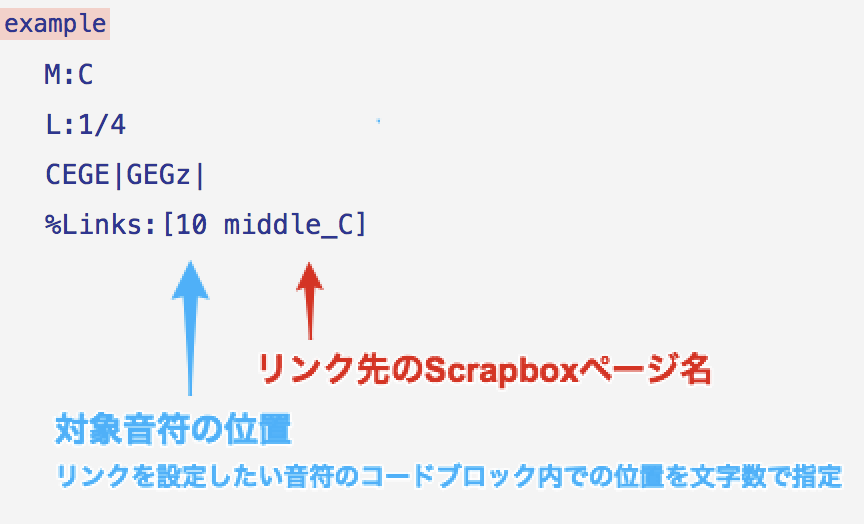
\includegraphics[width=10cm]{images/linkabc.png}
\caption{1音目の「C」に「middle C」ページへのリンクが設定されたABC}
\label{linkabc}
\end{figure}

\begin{figure}[H]
\centering
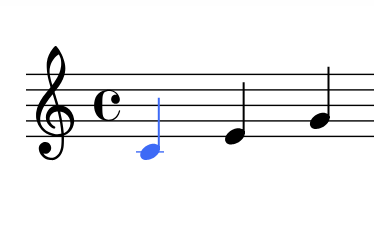
\includegraphics[width=4cm]{images/linkednote.png}
\caption{ハイパーリンクが設定された音符}
\label{linkednote}
\end{figure}

\begin{figure}[H]
\centering
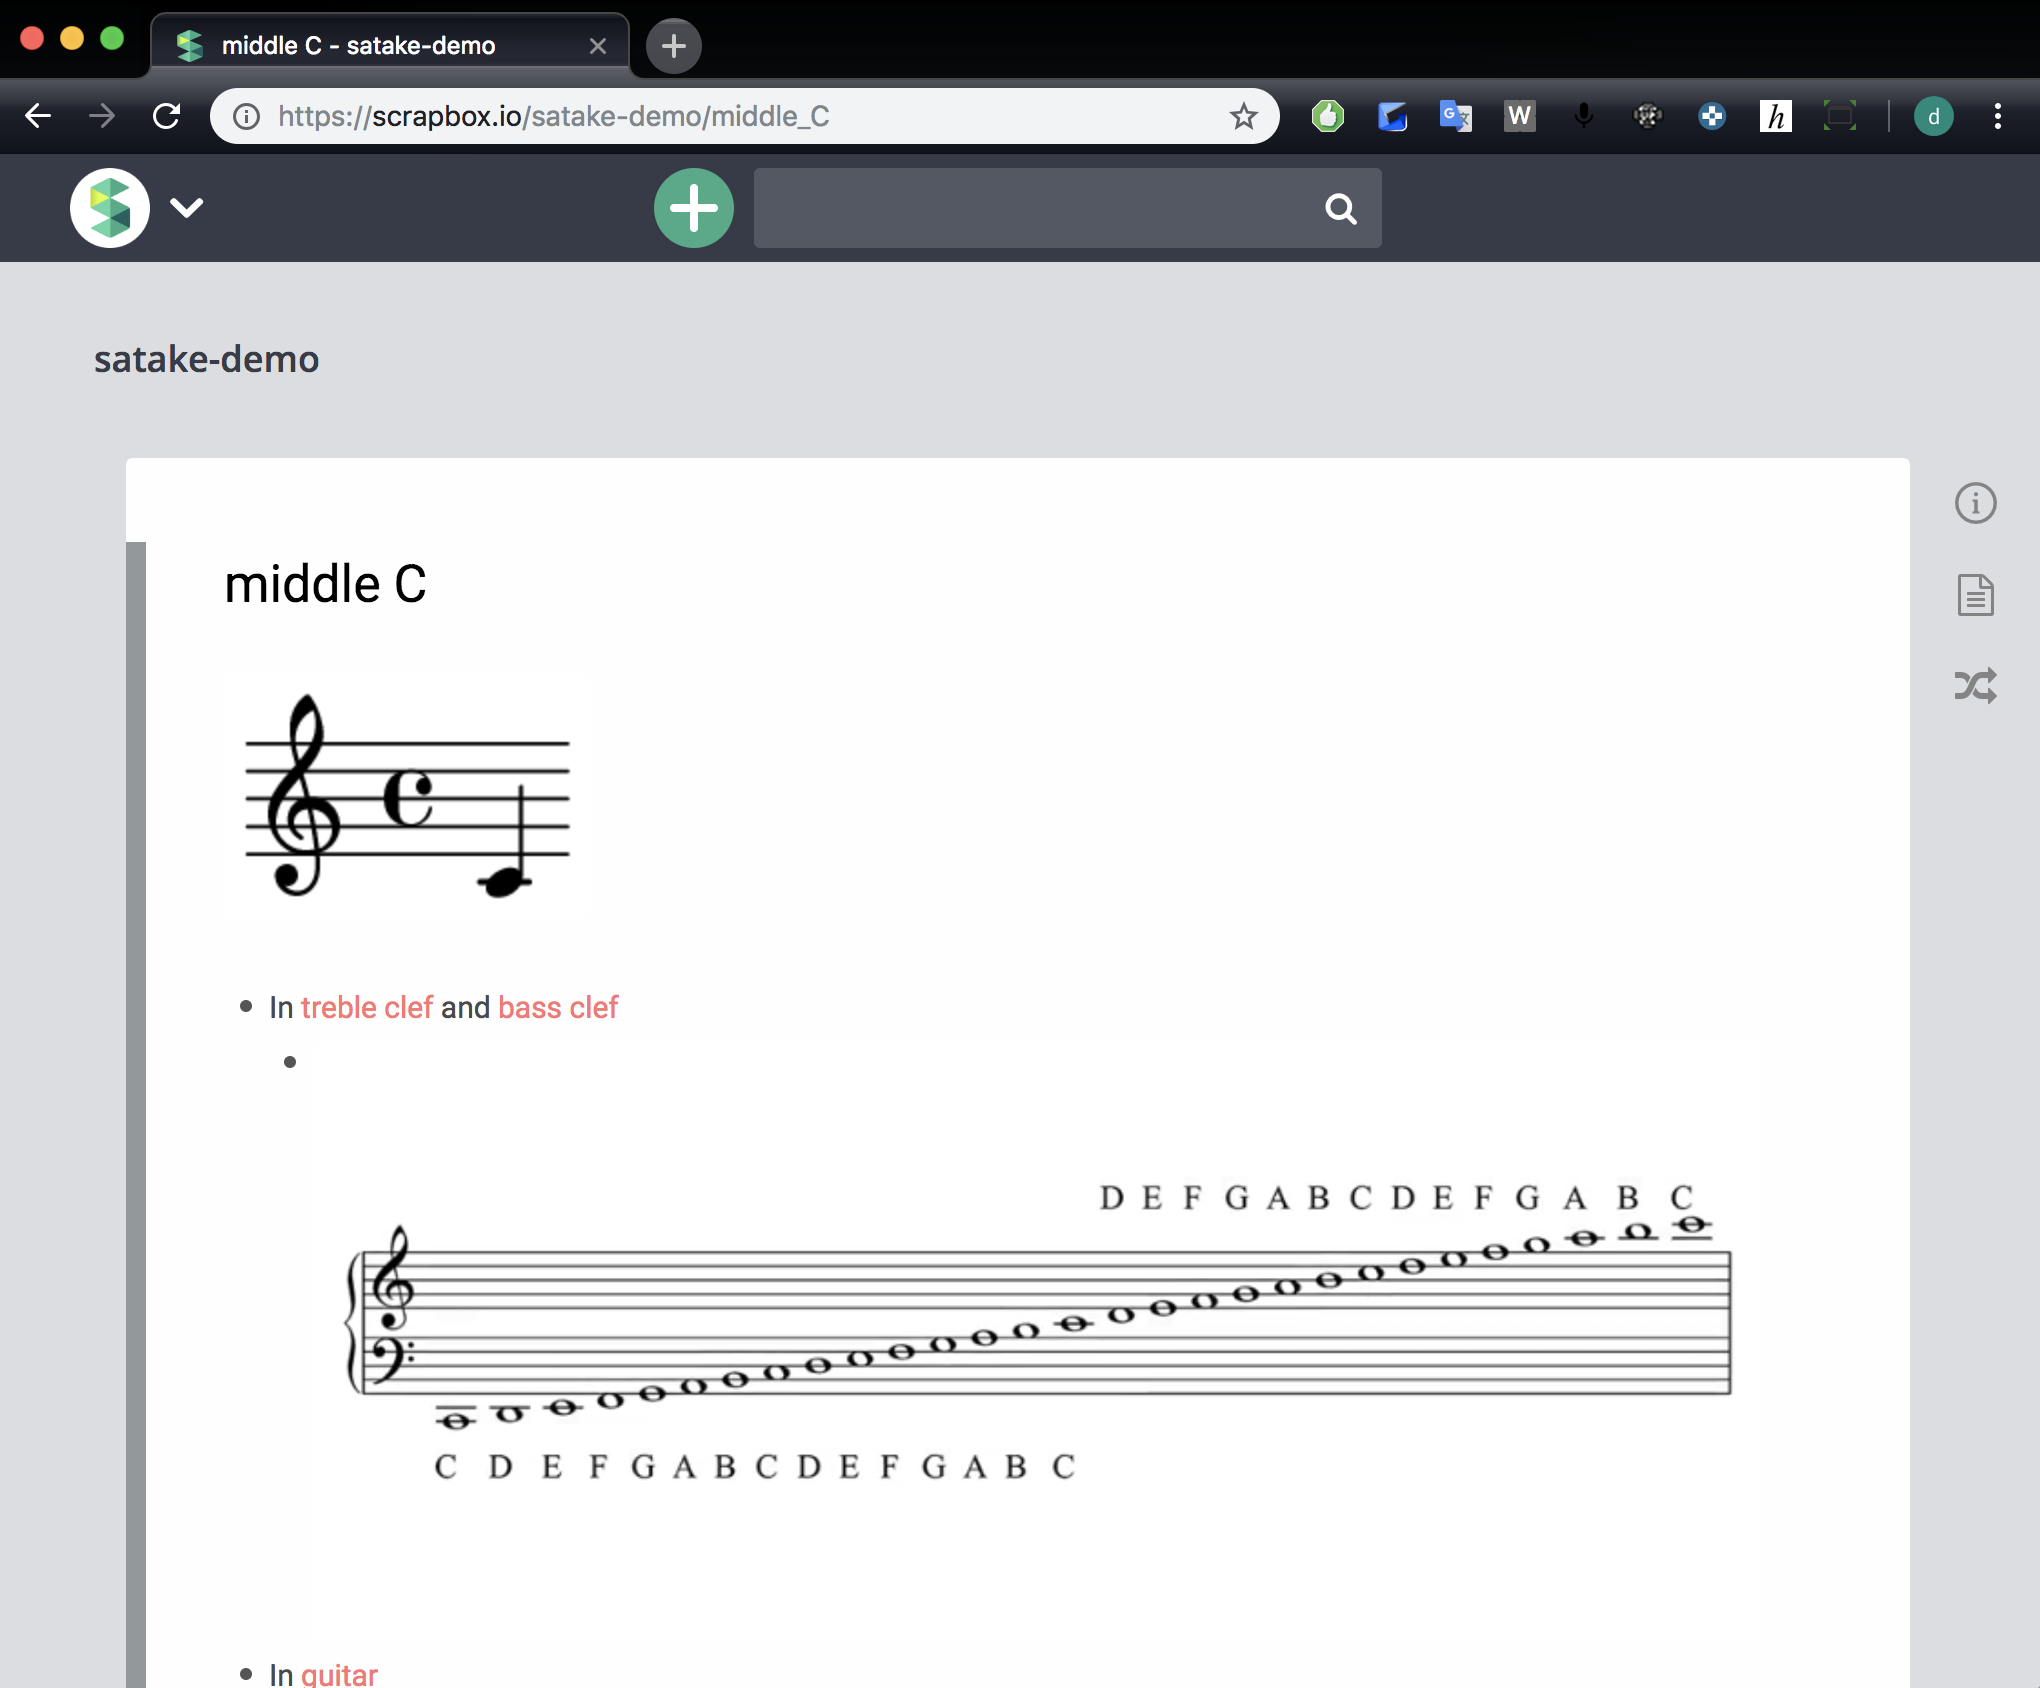
\includegraphics[width=10cm]{images/middlec.png}
\caption{リンク先の「middle C」ページ}
\label{middlec}
\end{figure}

